

\documentclass[11pt]{report}


% included packages
\usepackage{amsmath}
\usepackage{graphicx}
\usepackage{wrapfig}
\usepackage[autostyle]{csquotes}
\usepackage{amsfonts}
\usepackage[end]{algpseudocode}
\usepackage{caption}
\usepackage{setspace}
\usepackage{subcaption}
\usepackage{hyperref}
\usepackage[a4paper, total={6.25in, 8.5in}]{geometry}
\usepackage{algorithm}
\usepackage[all]{hypcap}
\usepackage{fontspec}
\usepackage{lipsum}
%\usepackage{tocbibind}
\usepackage{longtable}



% header/footer settings
\usepackage{fancyhdr}
\pagestyle{fancy}
\fancyhf{}
\fancyhead[R]{\rightmark}
\fancyhead[L]{\leftmark}
\fancyfoot[C]{\thepage}
\renewcommand{\headrulewidth}{0.5pt}
%\renewcommand{\sectionmark}[1]{\markright{#1}}
\renewcommand{\subsectionmark}[1]{}
\renewcommand{\subsubsectionmark}[1]{}



% polyglossia settings
\usepackage{polyglossia}
\setmainlanguage[numerals = maghrib]{arabic}
\setotherlanguage{english}

\setmainfont[Ligatures = TeX, Script = Arabic, Scale = 1]{Latin Modern Roman}
\setsansfont[Ligatures = TeX, Script = Arabic, Scale = 3]{Traditional Arabic}
\setmonofont[Ligatures = TeX, Script=Arabic, Scale = 3]{Traditional Arabic}
\newfontfamily\arabicfont[Script = Arabic, Ligatures = TeX, Scale = 1.5]{Traditional Arabic}
\newfontfamily\englishfont[Ligatures = TeX, Script = Latin, Scale = 1.15]{Latin Modern Roman}

%\setmainfont[Ligatures = TeX, Script = Arabic, Scale = 1]{Latin Modern Roman}
%\setsansfont[Ligatures = TeX, Script = Arabic, Scale = 3]{Traditional Arabic}
%\setmonofont[Ligatures = TeX, Script=Arabic, Scale = 3]{Traditional Arabic}
%\newfontfamily\arabicfont[Script = Arabic, Ligatures = TeX, Scale = 1.6]{Scheherazade}
%\newfontfamily\englishfont[Ligatures = TeX, Script = Latin, Scale = 1.15]{Latin Modern Roman}
%\DeclareMathSizes{18.7}{200}{16.59}{13.82}



% fixing parentheses in equations' numbering
\renewcommand{\theequation}{\arabic{equation}}
\makeatletter
\def\maketag@@@#1{\hbox{\m@th\normalfont\LRE{#1}}}
\def\tagform@#1{\maketag@@@{(\ignorespaces#1\unskip)}}
\makeatother



% fixing section/figure numbering
\renewcommand{\thesection}{\arabic{section}.\arabic{chapter}}
\renewcommand{\thesubsection}{\arabic{subsection}.\arabic{section}.\arabic{chapter}}
\renewcommand{\thesubsubsection}{\arabic{subsubsection}.\arabic{subsection}.\arabic{section}.\arabic{chapter}}
\renewcommand{\thefigure}{\arabic{figure}.\arabic{chapter}}



% setting chapter numbering to words
\newcommand\words[1]{\expandafter\xwords\csname c@#1\endcsname}
\def\xwords#1{\ifcase#1\or
	الأول\or          
	الثاني\or          
	الثالث\or 
	الرابع\or 
	الخامس\or 
	السادس\or 
	السابع\or 
	الثامن\or 
	التاسع\or 
	العاشر\or 
	الحادي عشر\or 
	الثاني عشر\or 
	الثالث عشر\or 
	الرابع عشر\or 
	الخامس عشر\or 
	السادس عشر\or  
	السابع عشر\or
	الثامن عشر\or 
	التاسع عشر\or 
	العشرون\or 
	\else
	أحتاج إلى المزيد من الأرقام!!!
	 \fi
}
\makeatletter
\patchcmd{\@makechapterhead}{\thechapter}{\words{chapter}}{}{}
\makeatother


% fixing footnoterule orientation
\renewcommand{\footnoterule}{%
	\kern-3pt
	\nointerlineskip
	\moveright.6\columnwidth\vbox{\hrule width.4\columnwidth}%
	\nointerlineskip
	\kern2.6pt
}



% references settings
\usepackage[
backend = biber,
sorting = ynt,
%style = authoryear,
%citestyle=authoryear
%language = english,
%autolang = langname, % never use this with polyglossia, there seem to be a bug
bibstyle=numeric,
style = numeric
]{biblatex}
\addbibresource{tex/references.bib}
%\AtEveryBibitem{\clearfield{pages}}





% preferences settings
\setlength{\parskip}{1em}
\setlength{\parindent}{0em}
\renewcommand{\baselinestretch}{1.5}
\hypersetup{colorlinks = true, allcolors = black} % change links colors
\captionsetup[figure]{name={الشكل}}
\addto\captionsarabic{\renewcommand{\chaptername}{الفصل}}
\newcommand{\eng}[1]{\textenglish{#1}}



% custom math commands definition
\newcommand{\argmax}{\operatornamewithlimits{argmax}}
\newcommand{\argmin}{\operatornamewithlimits{argmin}}
\newcommand{\norm}[1]{\left\lVert#1\right\rVert_{2}}
\newcommand{\pospart}[1]{\left\lfloor#1\right\rfloor_{+}}
\newcommand{\abs}[1]{\left\vert#1\right\vert}





\begin{document}
	
	% cover page
	

%\begin{titlepage}
	\thispagestyle{empty}
	\addcontentsline{toc}{chapter}{الغلاف}
	
	\newfontfamily\coverfont[Script = Arabic, Ligatures = TeX, SizeFeatures={Size=16}]{Traditional Arabic}
	\newfontfamily\authorsfont[Script = Arabic, Ligatures = TeX, SizeFeatures={Size=18}]{Traditional Arabic}
	
	{
		\begin{wrapfigure}{l}{0.25\textwidth}
			\hfill
			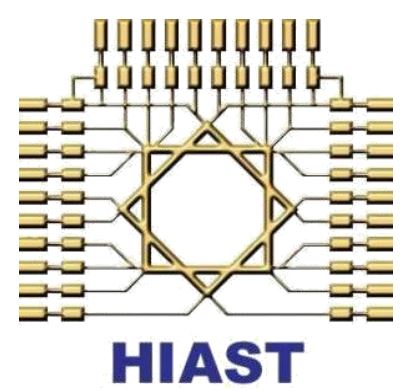
\includegraphics[width=0.9\linewidth]{images/HIAST_logo.JPG}
		\end{wrapfigure}
			
		\coverfont
		\begin{spacing}{1.8}
			\ \\
			الجمهورية العربية السورية \\
			المعهد العالي للعلوم التطبيقية والتكنولوجيا \\
			قسم المعلوميات \\
			العام الدراسي 2017/2018  \\
		\end{spacing}
	}
	
	
	\vspace{2cm}
	\begin{center}
		{
			\Huge
%			تقييم جودة نصوص اللغة الانكليزية

%			بناء مُصنّف لتقييم سهولة قراءة نصوص اللغة الانكليزية 
%			وفق عدّة مستويات باستخدام تعلم الآلة

			نظام خبير لتقييم مقروئية نصوص اللغة الانكليزية وفق عدّة مستويات
			\\[2.5mm]
			\Large
			مشروع السنة الرابعة
		}
	
		\vspace{3cm}
		\begin{doublespace}
			إعداد \\
			{
				\authorsfont
				فاروق حجابو \\[7mm]
			}
			إشراف \\[3mm]
			{
				\authorsfont
				د. غيداء ربداوي
				\hspace{2.5cm}
				م. رياض سنبل
			}
		\end{doublespace}
	\end{center}
		
	\vfill
	\centerline{2 أيلول 2018}
	
%\end{titlepage}



	
	
	% front matter
	\pagenumbering{roman}
	

\section*{الملخص}
\addcontentsline{toc}{section}{الملخص}
تُعد القراءة نشاط مهم نمارسه في حياتنا اليومية،
سواء للمطالعة أو قراءة الأخبار أو التعلم أو غيرها.
فيهتم هذا المشروع ببناء مُصنّف قادر على تقييم مقروئية النصوص المكتوبة باللغة الانكليزية.
وتصنيفها وفق عدّة مستويات (سهل، متوسط، صعب).
علماً بأن عدد هذه المستويات والتباين بين صعوبتها يتعلق بالمعطيات التي تم استخدامها لبناء هذا المصنّف.
تتمحور منهجية العمل حول استخراج مجموعة من السمات من هذه النصوص.
سمات تقليدية (مثل طول النص)، ومفرداتية (تعبّر عن تنوع المفردات المستخدمة)، ونحوية (تعكس الصياغة والتراكيب المستخدمة).
ثمّ استخدام خوارزميات تعلم الآلة (تم استخدام الـ \eng{SVM} بشكل أساسي) لتدريب وبناء مصنّف باستخدام هذه السمات.
تم استخدام مجموعة المعطيات \eng{One Stop English Corpus} والحصول على نسبة صِحّة $80.83\%$.
علماً أن أعلى نسبة صِحّة تم الحصول عليها باستخدام هذه المعطيات هي $78.13\%$.
وأيضاً خلال المشروع تم بناء مكتبة بلغة جافا لاستخراج السمات من النصوص.
فيمكن بسهولة استخدامها لاستخراج السمات التي تم تنجيزها من نص ما، أو توسيع هذه المكتبة بتعريف سمات جديدة.


\vfill
\selectlanguage{english}
\section*{Abstract}

Reading is an important activity in our daily lives.
We read the news, we read to learn, etc.
This project aims to build a classifier to automatically assess text readability for texts written in English.
By classifying them into different levels (easy, medium, and hard).
Noting that, the number of levels and the variance of their difficulties depends on the data used to build the classifier.
The methodology is to extract certain set of features from these texts.
Traditional features (e.g. text length), lexical features (measure vocabulary being used),
and syntactic features (measure sentence complexity).
Then using machine learning algorithms (SVM mainly) to train and build a classifier using these features.
Using One Stop English Corpus as the dataset, we achieved an accuracy of $80.83\%$.
Given that the best achieved accuracy on this dataset is $78.13\%$.
Also, we implemented a library in java to extract features from texts.
It can be easily used to extract the features we implemented from a given text.
It also can be extended by implementing new features.

\selectlanguage{arabic}






	
	
	% indexes/contents
	\tableofcontents
	\addcontentsline{toc}{chapter}{المحتويات}
	
	\listoffigures
	\addcontentsline{toc}{chapter}{قائمة الأشكال}
	
	\listoftables
	\addcontentsline{toc}{chapter}{قائمة الجداول}
	
	
	% main matter
	\pagenumbering{arabic}
	

\chapter{التعريف بالمشروع}
يُمهّد هذا الفصل للمشروع، حيث يُبيّن فكرة المشروع وأهميتها والأهداف المرجوّة منه. ويذكر المتطلبات الوظيفية وغير الوظيفية للمشروع.

\section{مقدمة}
تعتبر القراءة والمطالعة واحدة من أكثر الطرق المستخدمة للتعلم واكتساب المعارف.
وبالتالي فإن العوامل الت


	
	
	% bibliography/references
	\nocite{*}
	
	\printbibheading[title = {المراجع}]
	\addcontentsline{toc}{chapter}{المراجع}
		
		{
			\setmainfont[Script = Latin]{Traditional Arabic}
			\setsansfont[Script = Latin]{Traditional Arabic}
			\selectlanguage{english}
%			\print‌​bibliography[notkeyword‌​={arabic}, title={test}, heading=subbibliography]
\begin{LTR}
		\printbibliography[heading = subbibliography, notkeyword = arabic, title = {English References}]
		\end{LTR}
		}
	
%	\begin{english}
%		
%		\printbibliography[heading = subbibliography, notkeyword = arabic, title = {English References}]
%	\end{english}
	
%	\printbibliography[heading = subbibliography, keyword = arabic, title = {المراجع العربية}]
	
			{
		\setmainfont[Script = Arabic]{Traditional Arabic}
		\setsansfont[Script = Arabic]{Traditional Arabic}
		\selectlanguage{arabic}
		%			\print‌​bibliography[notkeyword‌​={arabic}, title={test}, heading=subbibliography]

\begin{RTL}
	\printbibliography[heading = subbibliography, keyword = arabic, title = {المراجع العربية}]
	\end{RTL}
	}
\end{document}



